\documentclass[12pt,a4paper]{scrartcl}
\usepackage[T1]{fontenc}
\usepackage[latin1]{inputenc}
\usepackage{graphicx}
\usepackage{hyperref}
\usepackage{fancyref}
\usepackage[ngerman]{babel}
\usepackage{times}
\usepackage{listings}
\usepackage{xcolor}


\definecolor{codegreen}{rgb}{0,0.6,0}
\definecolor{codegray}{rgb}{0.5,0.5,0.5}
\definecolor{codepurple}{rgb}{0.58,0,0.82}
\definecolor{backcolour}{rgb}{0.95,0.95,0.92}

\lstdefinestyle{code}{
	backgroundcolor=\color{backcolour},   
    commentstyle=\color{codegreen},
    keywordstyle=\color{magenta},
    numberstyle=\tiny\color{codegray},
    stringstyle=\color{codepurple},
    basicstyle=\ttfamily\footnotesize,
    breakatwhitespace=true,         
    breaklines=true,                 
    captionpos=b,                    
    keepspaces=true,                 
    numbers=left,                    
    numbersep=5pt,                  
    showspaces=false,                
    showstringspaces=false,
    showtabs=false,                  
    tabsize=2
}
\lstset{style=code}

\title{Semesterprojekt \\ Neuronales Netz} 
\author{\\\\\\\\\\\\\\\\\\\\\\\\\\\\\\\\\
  Moritz Lechner\\
  Konstantin Ro\ss mann\\
  Leon Sobotta\\\\
  Mikroprozessortechnik\\
  Computer Engineering
}


\date{\today}


\begin{document}


\maketitle

\pagebreak

\tableofcontents
\listoffigures	

\pagebreak


\section{Einleitung}

F"ur diese Seminararbeit sollte ein funktionierendes neuronales Netz von Grund auf konstruiert werden, welches letztendlich in der Lage ist, handschriftliche Zahlen zu erkennen. Das sollte ohne externe Bibliotheken in den Sprachen C oder C++ realisiert werden. Da dieser Prozess viel Rechenleistung erfordert, sollte das Programm zus"atlich in zwei Varianten mit Parallelverarbeitung implementiert werden.\\

Damit der Algorithmus die handschriftlichen Zahlen "uberhaupt erkennen kann, muss er diese wie ein Mensch zuerst lernen. Dabei spricht man von maschinellen Lernen. Der Computer, also genauer der Algorithmus, lernt dabei Zusammenh"ange zwischen dem Input und dem erw"unschten Ergebnis zu erkennen. Ein Mensch kann in etwa ab dem 2. Lebensjahr  z"ahlen und entwickelt mit ungef"ahr 4 Jahren eine Zahlenverst"andnis. Damit der Algorithmus nicht so lange braucht, daher lohnt es sich diesen zu beschleunigen. \\

Diese Parallelisierung sollte die Laufzeit des Programms im Vergleich zur sequentiellen Implementierung deutlich verk"urzen (\textit{Speedup}). Theoretisch lie\ss e sich die Laufzeit mit doppelt so vielen genutzten Kernen halbieren, dass jedoch nur wenn wirklich das gesamte Programm parallelisiert werden kann. Das wird beim neuronalen Netz voraussichtlich aber nicht umsetzbar sein, da gewisse Teile auf Ergebnisse von vorherigen Berechnungen warten m"ussen. Dennoch sollte sich die Laufzeit des Algorithmus deutlich verk"urzen lassen.\\

Zur Umsetzung wurde OpenMP genutzt und die Compiler Version \textit{SIMD} gew"ahlt. Als Programmiersprache wurde vor allem C benutzt, da sich mit C sehr genau programmieren l"asst, es werden keine unbekannten oder ungewollte Funktionen im Hintergrund ausgef"uhrt. 


\section{Grundlagen von Neuronalen Netzen}

Neuronale Netze sind beliebig viele verbundene Neuronen und sind damit Teil eines Nervensystems, sie sind also wichtige Objekte in der Biologie. Ihre Arbeitsweise hat man sich in der Informatik zu nutzen gemacht, wo man k"unstliche Neuronale Netze entwickelt, um Aufgaben zu l"osen bei denen normale Programme an ihre Grenzen sto\ss en. "Ahnlich wie das Menschliche Gehirn k"onnen k"unstliche Neuronale Netze in gewisser Weise lernen, somit eignen sie sich perfekt f"ur Aufgaben bei denen man Entscheidungen treffen muss, und auf Basis der vorherigen Erfahrungen die nachfolgenden Ergebnisse anpassen kann. Das sind zum Beispiel Bild- und Stimmenerkennung, Maschinelles "Ubersetzen, Chatbots, autonomes Fahren oder die Robotik\footnote{siehe Quelle \ref{ki_einsatz}}.\\

\pagebreak

Ein solches Netz besteht aus mehreren Schichten von Neuronen, wie in Abbildung \ref{einfaches_netz} zu sehen ist. Dabei gibt es immer mindestens eine Eingabe- und eine Ausgabeschicht, die von mindestens einer versteckten Schicht getrennt sind. Diese versteckten Schichten sind es, die dem Netz seine F"ahigkeit zum lernen geben, je mehr ein Netz besitzt, desto komplexer kann es werden. Die einzelnen Schichten bestehen aus Neuronen die von Schicht zu Schicht miteinander verbunden sind um Daten weiterzugeben. Werden die Inputs in einem Netz von der ersten zur letzten Schicht immer weitergegeben, wird dieses Netz als \textit{feed forward} Netz bezeichnet. Mittlerweile werden die meisten neuronalen Netze auf diese Weise realisiert, so auch unseres.\\

\begin{figure}[h]
	\centering
	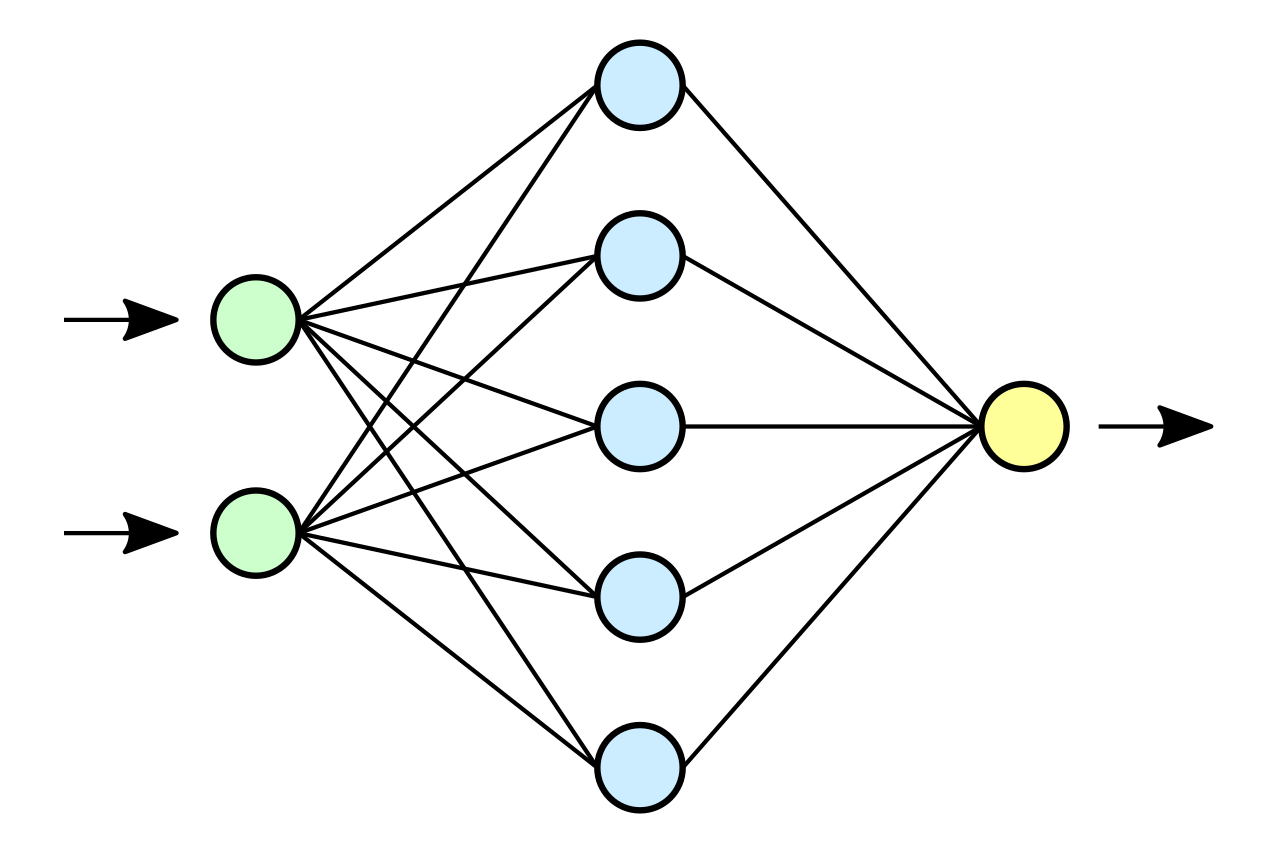
\includegraphics[width=10cm]{screens/neural_net.png}
	\caption{Ein vereinfachtes Neuronales Netz bestehend aus Neuronen. Quelle: Wikipedia} \label{einfaches_netz}
\end{figure}


In der Abbildung \ref{schema_net} kann man sehen, dass jedes Neuron aus den Gewichtungen, der "Ubertragungsfunktion und der Aktivierungsfunktion besteht. Die Gewichtungen sind Faktoren, mit denen die Eingaben der vorherigen Neuronen multipliziert werden. Diese gewichteten Eingaben werden dann in der "Ubertragungsfunktion zur Netzeingabe zusammengefasst und schlie\ss lich durch die Aktivierungsfunktion zur Ausgabe dieses Neurons, welches den Wert an die n"achste Schicht weitergibt, bis man an der Ausgabeschicht angekommen ist. Wenn das errechnete Ergebnis nicht mit den Erwartungen "ubereinstimmt, wird eine Fehlerfunktion angewendet, welche bestimmt, ob die Gewichtungen vergr"o\ss ert oder verringert werden sollen, das nennt sich \textit{Fehlerr"uckf"uhrung}. Wie stark die Gewichte angepasst werden, also wie gro\ss\ die Lernfaktoren sind, wird mit der \textit{Backpropagation} \label{backprop_text} berechnet. Dabei wird die Kostenfunktion ben"otigt, welche angibt wie genau die Vorhersagen des Netzes sind. Je gr"o\ss er sie ist, desto ungenauer ist das Netz, dementsprechend m"ochte man den Punkt finden, an dem sie nahezu null ist, was mit Hilfe der Ableitung und den entsprechenden Gewichten passiert. Zuerst werden die Anpassungen f"ur die letzte Schicht vorgenommen, dann werden die Schichten von hinten nach vorne darauf basierend angepasst. Jede Anpassung beruht auf der vorherigen, somit werden doppelte Berechnungen minimiert und der Algorithmus l"auft schneller. Das macht bei einem kleinen Netz wie unserem keinen gro\ss en Unterschied, doch bei komplexeren Strukturen ist dieses Vorgehen unverzichtbar. \\

\begin{figure}[h]
	\centering
	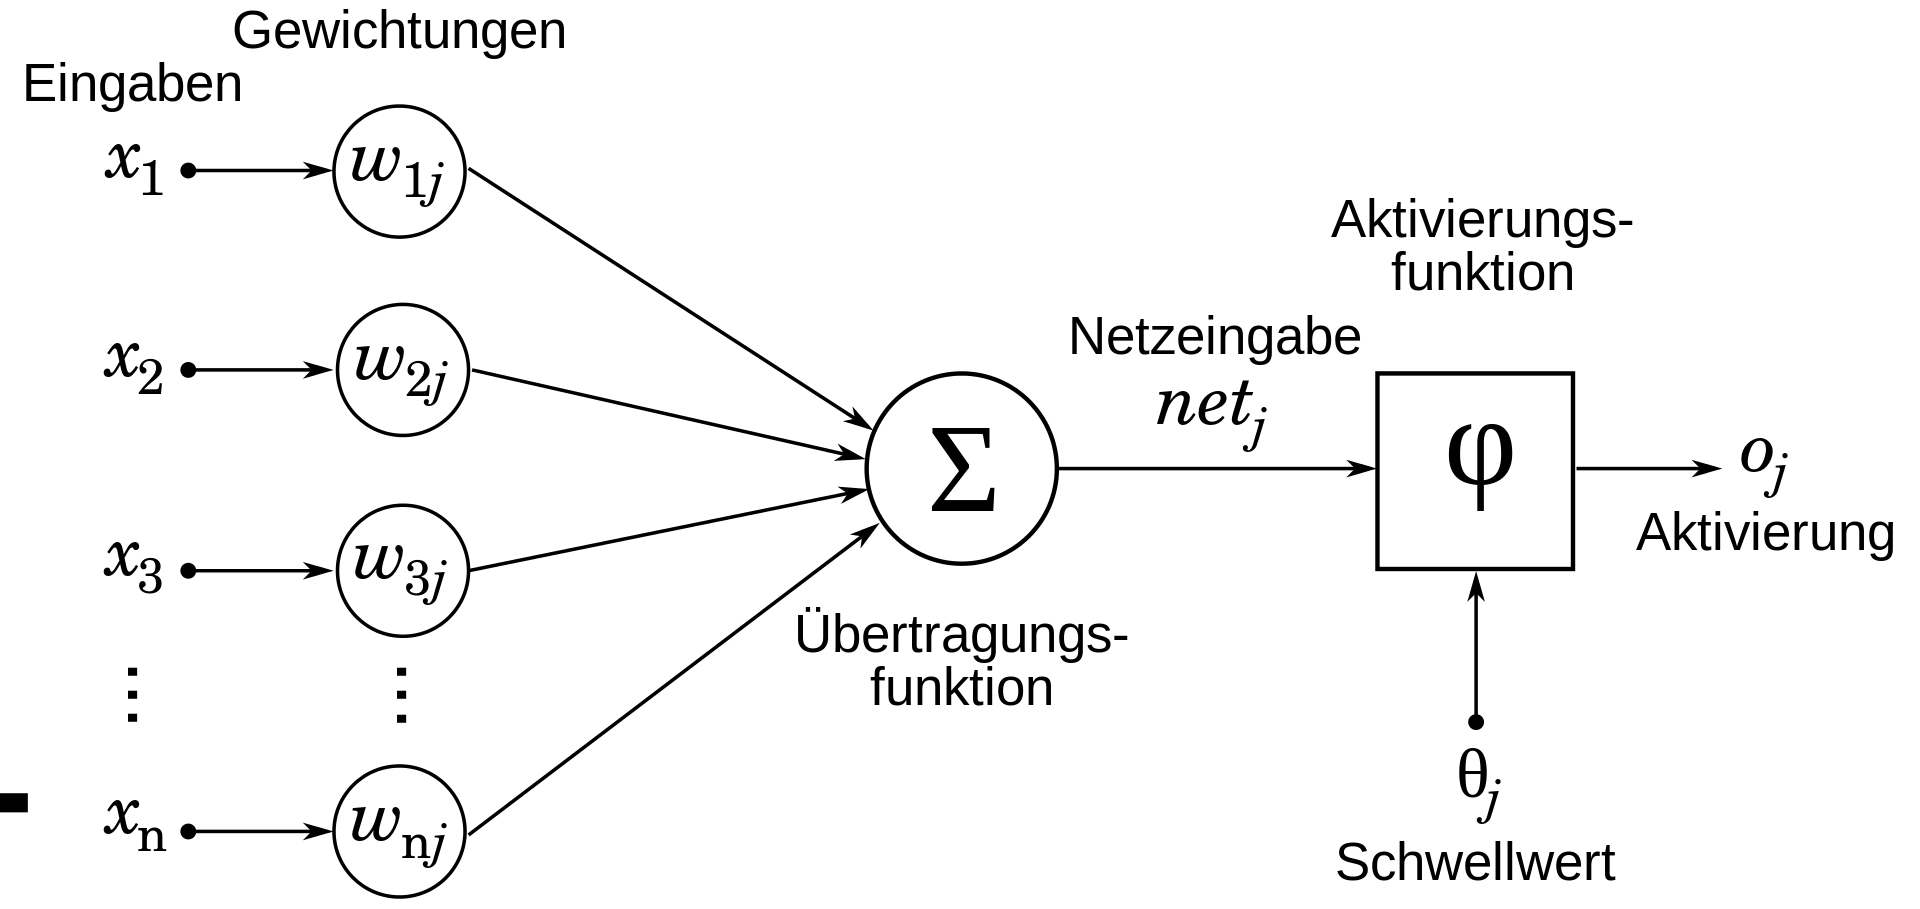
\includegraphics[width=9cm]{screens/schema_net.png}
	\caption{Das Schema eines k"unstlichen Neurons. Quelle: Wikipedia} \label{schema_net}
\end{figure}


Um ein neuronales Netz zu nutzen muss man es zuerst trainieren, daf"ur greift das Netzwerk auf eine enorme Datenmenge von mehreren Tausend Datens"atzen zur"uck. F"ur diese berechnet das Netz dann seine Ausgabe, vergleicht diese mit dem erwarteten Ergebnis, den \textit{Label Daten}, und passt gegebenenfalls seine Gewichtungen an. Nachdem sich das Netz durch s"amtliche Trainingsdaten durchgearbeitet hat wird es an einem kleineren Testdatensatz getestet, es gibt also wieder Ausgaben, doch diesmal lernt es dabei nicht. Da selbst die vielen Beispiele aus den Trainingsdaten oft nicht reichen um eine hohe Genauigkeit zu erzielen, f"angt das Netz dann erneut an die Daten durchzugehen, diesmal aber nicht mit zuf"alligen Gewichtungen, sondern mit den bereits verbesserten. Jeder dieser Durchl"aufe ist eine neue Epoche des Netzwerkes.


\subsection{Grundlagen unseres Netzes}

In der ersten funktionierenden Version hatte unser Netz nur eine Eingabe- und eine Ausgabeschicht. Es handelte sich also noch um ein sehr simples Netzwerk, das Perceptron (siehe Abbildung \ref{perceptron_pic}), und ebenso simpel war auch die Berechnung der Lernfaktoren, welche mit der \textit{Delta Learn Regel} \label{deltalearn_text} \footnote{siehe Quelle: \ref{delta_learn_wiki}} berechnet wurden.\\

Diese Berechnet die Anpassung der Gewichte unter der Zuhilfenahme der Lernrate $\epsilon $, der Differenz aus der erwarteten Ausgabe $t_j$ und der tats"achlichen Ausgabe $y_j$ sowie der entsprechenden Eingabe $x_i$. Das alles wird in folgender Formel zusammengefasst: 

$$ \Delta w_{ji} = \epsilon(t_j - y_j)x_i $$

Mithilfe der Lernrate kann einerseits die Geschwindigkeit des Lernprozesses, andererseits aber auch die Genauigkeit kontrollieren kann. Je gr"o\ss er die Lernrate, desto gr"o\ss er sind auch die Schritte, mit denen das Netz lernt. Das Problem ist, dass man mit gro\ss en Spr"ungen das Optimum verfehlen kann. Daher nutzt man eher einen Wert irgendwo in der Mitte, bei unserem Perceptron hat sich eine Lernrate von 0,1 als am effektivsten herausgestellt. Die Lernrate ist in der Regel umgekehrt proportional zur Gr"o\ss e des Netzes.\\

Das Perceptron oder auch One Layer Neural Net verh"alt sich dabei sehr "ahnlich wie die Linear Regression und kann daher nur in einem bestimmten Breich der Standardabweichung Zusammenh"ange erkennen. Dadurch ist die Genauigkeit auch deutlich niedriger als in einem komplexeren Neuronalen Netz.\\

\begin{figure}[h]
	\centering
	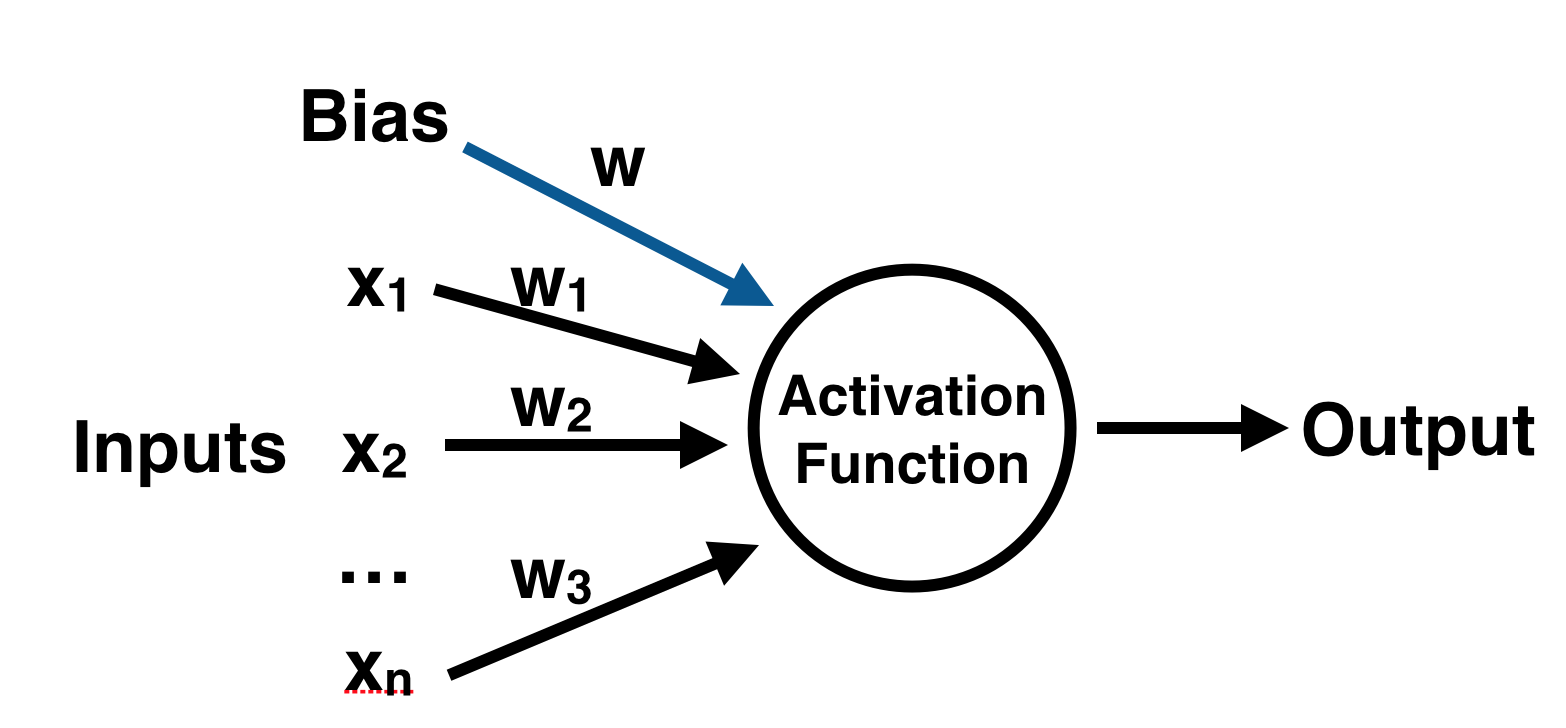
\includegraphics[width=10cm]{screens/perceptron.png}
	\caption{Darstellung eines Perceptrons} \label{perceptron_pic}
\end{figure}

Mit diesem Aufbau lie\ss sich "uberraschender Weise innerhalb von 50 Epochen bereits eine Genauigkeit von "uber 90 \% erreichen. Als wir dann jedoch versucht haben eigene Beispiele von Zahlen durch das Netz erkennen zulassen hatte es eine deutlich schlechtere Genauigkeit. Wir haben das auf die geringe Varianz der Zahlen des Datensatzes zur"uckgef"uhrt, mit denen es gelernt hat. \\

In der n"achsten Entwicklungsstufe wird unser Netzwerk um eine Schicht erweitert und besteht nun aus einer Eingabeschicht, zwei versteckten Schichten und einer Ausgabeschicht. Dabei hat die Eingabeschicht 784 Neuronen, da die Bilder der Zahlen in 28 $\cdot$ 28 Pixeln aufl"osen. Die versteckten Schichten haben 16 bzw. 10 und die Ausgabeschicht hat 10 Neuronen, f"ur jede der m"oglichen Antworten eins. F"ur den ersten Durchlauf werden die Gewichtungen zuf"allig generiert. Die "Ubertragungsfunktion unseres Netzes ist ein einfaches Kreuzprodukt aus den Gewichten und den Eingaben:

$$ a \times b = 	\sum_{n=1}^{N} a[i] \cdot b[i] $$

Als Aktivierungsfunktion nutzen wir die Sigmoidfunktion, allerdings ohne Vorfaktor. Diese Funktion ist als Aktivierungsfunktion sehr verbreitet, da sie sich in der "Ubergangsregion sehr gleichm"a\ss ig verh"alt und daher gut differenzierbar ist. Au\ss erdem gibt sie f"ur alle Eingaben einen Wert zwischen 0 und 1 aus, so dass s"amtliche Inputs in einen festen Wertebereich konvertiert werden. Der Graph, welcher diese Funktion beschreibt ist in Abbildung \ref{sigmoid} zu sehen. Die Funktion selbst lautet wie folgt:

$$ \frac{1}{1+e^{-x}}$$	

Durch das hinzuf"ugen der weiteren Schichten zwischen Input und Output, k"onnen nun nicht mehr einfach die Differenz zu dem gew"unschten Ergebniss mit der Gewichtung addiert werden. Die dadurch neu enstandenen Verbindungen lassen sich nicht mehr so leicht ver"andern und sind auch nicht mehr intuitiv mit der Wertigekeit der Eingabe und Ausgabe verbunden.\\

Um diese Gewichtungen nun auch richtig anpassen zu k"onnen m"ussen wir unsere Formel erweitern und eine Fallunterscheidung machen. Dabei helfen die Erkenntnis aus der Delta Learn Regel weiter hin. Den f"ur die Verbindungen, die in den Output f"uhren, ist $\Delta w_{ji}$ weiterhin direkt vom Output und dem erwarteten Wert abh"angig. Erst f"ur die folgenden Schichten muss die Formel angepasst werden. \\

Die Berechnung der Lernfaktoren mit der Backpropagation wird mit der folgenden Formel realisiert. Dabei entspricht $ z^l_j$ dem Faktor f"ur das Neuron \textit{j} in der Schicht \textit{l}, w"ahrend \textit{m}  f"ur die Anzahl an Schichten steht.

$$ z^l_j = \sum_{k=1} ^{m} w^l_{jk}a^{l-1}_k + b^l_j  $$

Beim Perceptron hatte jeder Output einen jeweiligen Fehler, um nun den Fehler der jedes Hidden Neurons zu berechnen, wird der Fehler des Outputs nach hinten gereicht. Dieser Fehler dient dabei als Richtung und gibt an ob eine Flanke erh"oht oder gesenkt werden muss. In der Hidden Schicht ergibt sich der Fehler aus der Summe der Fehler der vorherigen Schicht und der Wertigkeit der jeweiligen Verbindung mit der die Neuronen verbunden sind. So gibt jedes Output Neuronen seinen Fehler nach hinten, dort geben die Neuronen, dann mit Hilfe der gleichen Technik ihreren vorher berrechneten Fehler nachhinten und der Schritt wird so oft wiederholt, bis der Input erreicht wird. \\

Damit jede Anpassung nicht nur in die richtige Richtung sonder auch in der richtigen St"arke geschiet, muss bei jeder Anpassung auch die Relevanzen der Verbindungen betrachtet werden und als Faktoren mit eingrechnet werden. Dieser Faktoren ergeben sich einmal schon aus der gr"o\ss e der jeweiligen Fehler, denn umso st"arker die Abweichungen, umso st"arker k"onnen die Gewichtung angepasst werden. Die weiteren Faktoren sind die jeweiligen Inputs, die "uber die anzupassenden Gewichtung in das Neuron gegeben werden und der eigene Wert des Neurons. \\

\begin{figure}[h]
	\centering
	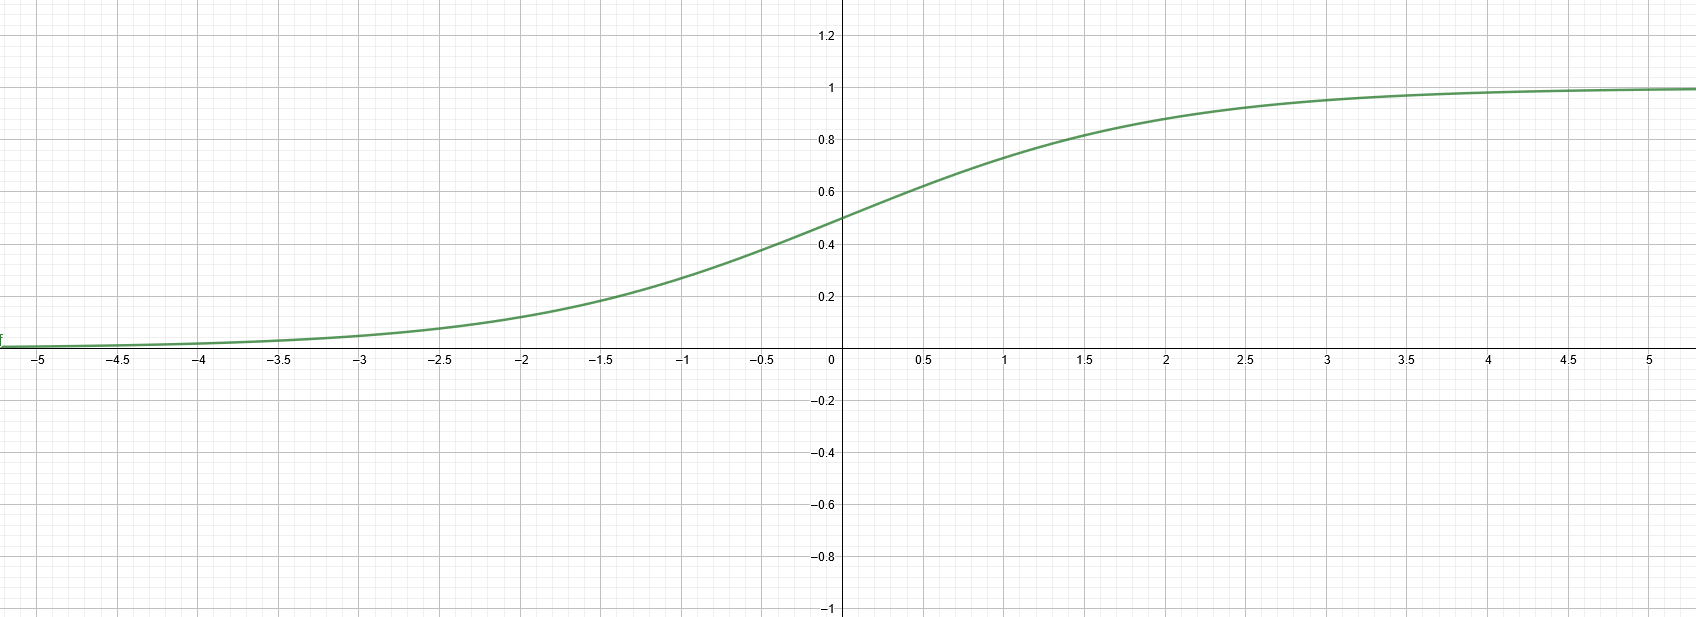
\includegraphics[width=14cm]{screens/wiki_sigmoid.png}
	\caption{Darstellung der Sigmoidfunktion} \label{sigmoid}
\end{figure}

Die von uns verwendeten Daten stammen aus dem weit verbreiteten MNIST-Datensatz\footnote{Modified National Institute of Standards and Technology database}, welcher aus 60.000 Trainingsdaten und 10.000 Testdaten besteht.

\pagebreak

\section{Vergleich Sequentiell zu Parallelisiert}

Wenn das Perceptron beispielsweise 200 Epochen sequentiell durchlaufen w"urde, m"usste man "uber 2 Minuten auf ein Ergebnis warten, das ist nicht sonderlich praktisch wenn man gewisse Parameter ausprobieren und anpassen m"ochte. Vor allem da das Programm mit steigender komplexit"at des Netzes und hinzuf"ugen der Packprogation noch langsamer wird. Daher muss man einen Weg finden um die Laufzeit des Programmes deutlich zu verk"urzen, ohne dabei die Komplexit"at und damit die Leistungsf"ahigkeit des Netzes zu verringern. Da man das Programm also nur sehr begrenzt simpler machen kann muss man die Abarbeitung effizienter gestalten, indem man das Programm parallel laufen l"asst. \\

Um diese Parallelisierung zu implementieren k"onnen verschiedene Methoden genutzt werden. F"ur unser Programm haben wir zum einen das Konzept \textit{Single Instruction Multiple Data} (\textit{SIMD}), sowie die Parallelisierung mit der C-eigenen Funktion \textit{omp parallel} genutzt. OMP bedeutet Open-Multi-Processing, dabei werden Schleifen in Programmen auf mehrere Threads\footnote{Teil eines Prozesses, der unabh"angig durchlaufen werden kann} aufgeteilt, so dass diese deutlich schneller abgearbeitet werden k"onnen. Wenn das Durchlaufen einer Schleife beispielsweise auf 8 Threads aufgeteilt wird, braucht dieser Prozess nur noch ein Achtel der Zeit. Bei SIMD wird das Programm weiterhin nur auf einem Kern ausgef"uhrt, dabei werden die Elemente der zu verarbeitenden Vektoren aber an mehrere ALUs (Arithmetic Logic Unit) verteilt und k"onnen so parallel auf \textit{Lanes} verarbeitet werden\footnote{siehe Quelle: \ref{bauer_simd}}. Da ein Vektor eine Reihe einzelner Werte vom gleichen Typ ist, kann die ALU sie als eine Einheit verarbeiten. Somit eignet sich dieses Verfahren gut f"ur Neuronale Netze, da Vektoren dort bei fast allen Berechnungen vorkommen.

\begin{figure}[h]
	\centering
	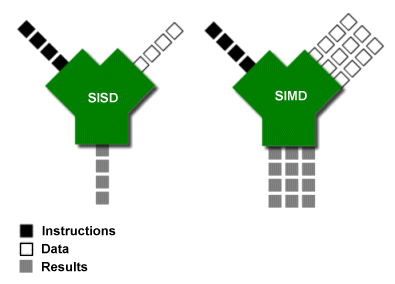
\includegraphics[width=10cm]{screens/ars_simd.png}
	\caption{Verbildlichung von SIMD. Quelle: arstechnica.com} \label{ars_simd}
\end{figure}

\pagebreak

\subsection{Darstellung der Ergebnisse}
Wir wollen nun unser neuronales Netz auf seine Genauigkeit und Laufzeit auswerten. Umgesetzt haben wir das, indem wir ein Python-Script geschrieben haben, welches das neuronale Netz automatisch mit stetig steigenden Epochen trainiert und getestet hat. Die daraus resultierenden Laufzeiten und Genauigkeiten wurden von dem Script zwischengespeichert und anschlie\ss end in anschaulichen Graphen dargestellt. Dieser Prozess wurde drei mal ausgef"uhrt, einmal f"ur die nicht parallelisierte Version, dann f"ur die mit OMP parallelisierte Version und anschlie\ss end f"ur die mit SIMD parallelisierte Version. \\

Als erstes Betrachten wir Laufzeit der verschiedenen Parallelisierungen in Abbildung \ref{runtime single}. In dem Graph ist sehr gut zu erkennen, dass die Laufzeit des Netzes ohne Parallelisierung bei einer niedrigen Anzahl an Epochen noch relativ nah bei der Laufzeit des parallelisierten Codes liegt. Dies "Andert sich jedoch im weiteren Verlauf des Graphen. Bereits bei 25 Epochen betr"agt die Differenz zwischen parallelisiert und nicht parallelisiert 25 Sekunden. Auch Auff"allig in dem Graph ist, dass die Laufzeit der mit OMP parallelisierten Version, der mit SIMD parallelisierten Version "ahnelt. Das l"asst sich dadurch erkl"aren, dass wir SIMD nicht richtig angewendet haben. Wir sind an dieser Stelle an unsere Grenzen gekommen und  wussten nicht wie wir SIMD korrekt implementieren sollen. Daher l"asst sich kein wirklich erkennbarer Unterschied zwischen diesen beiden Laufzeiten feststellen. Trotzdem haben wir, wie in der folgenden Abbildung \ref{speedup single} erkennbar, durch die Parallelisierung des Codes einen Speedup von im Schnitt 1.5 erreichen k"onnen.


\pagebreak

\begin{figure}[h]
	\centering
	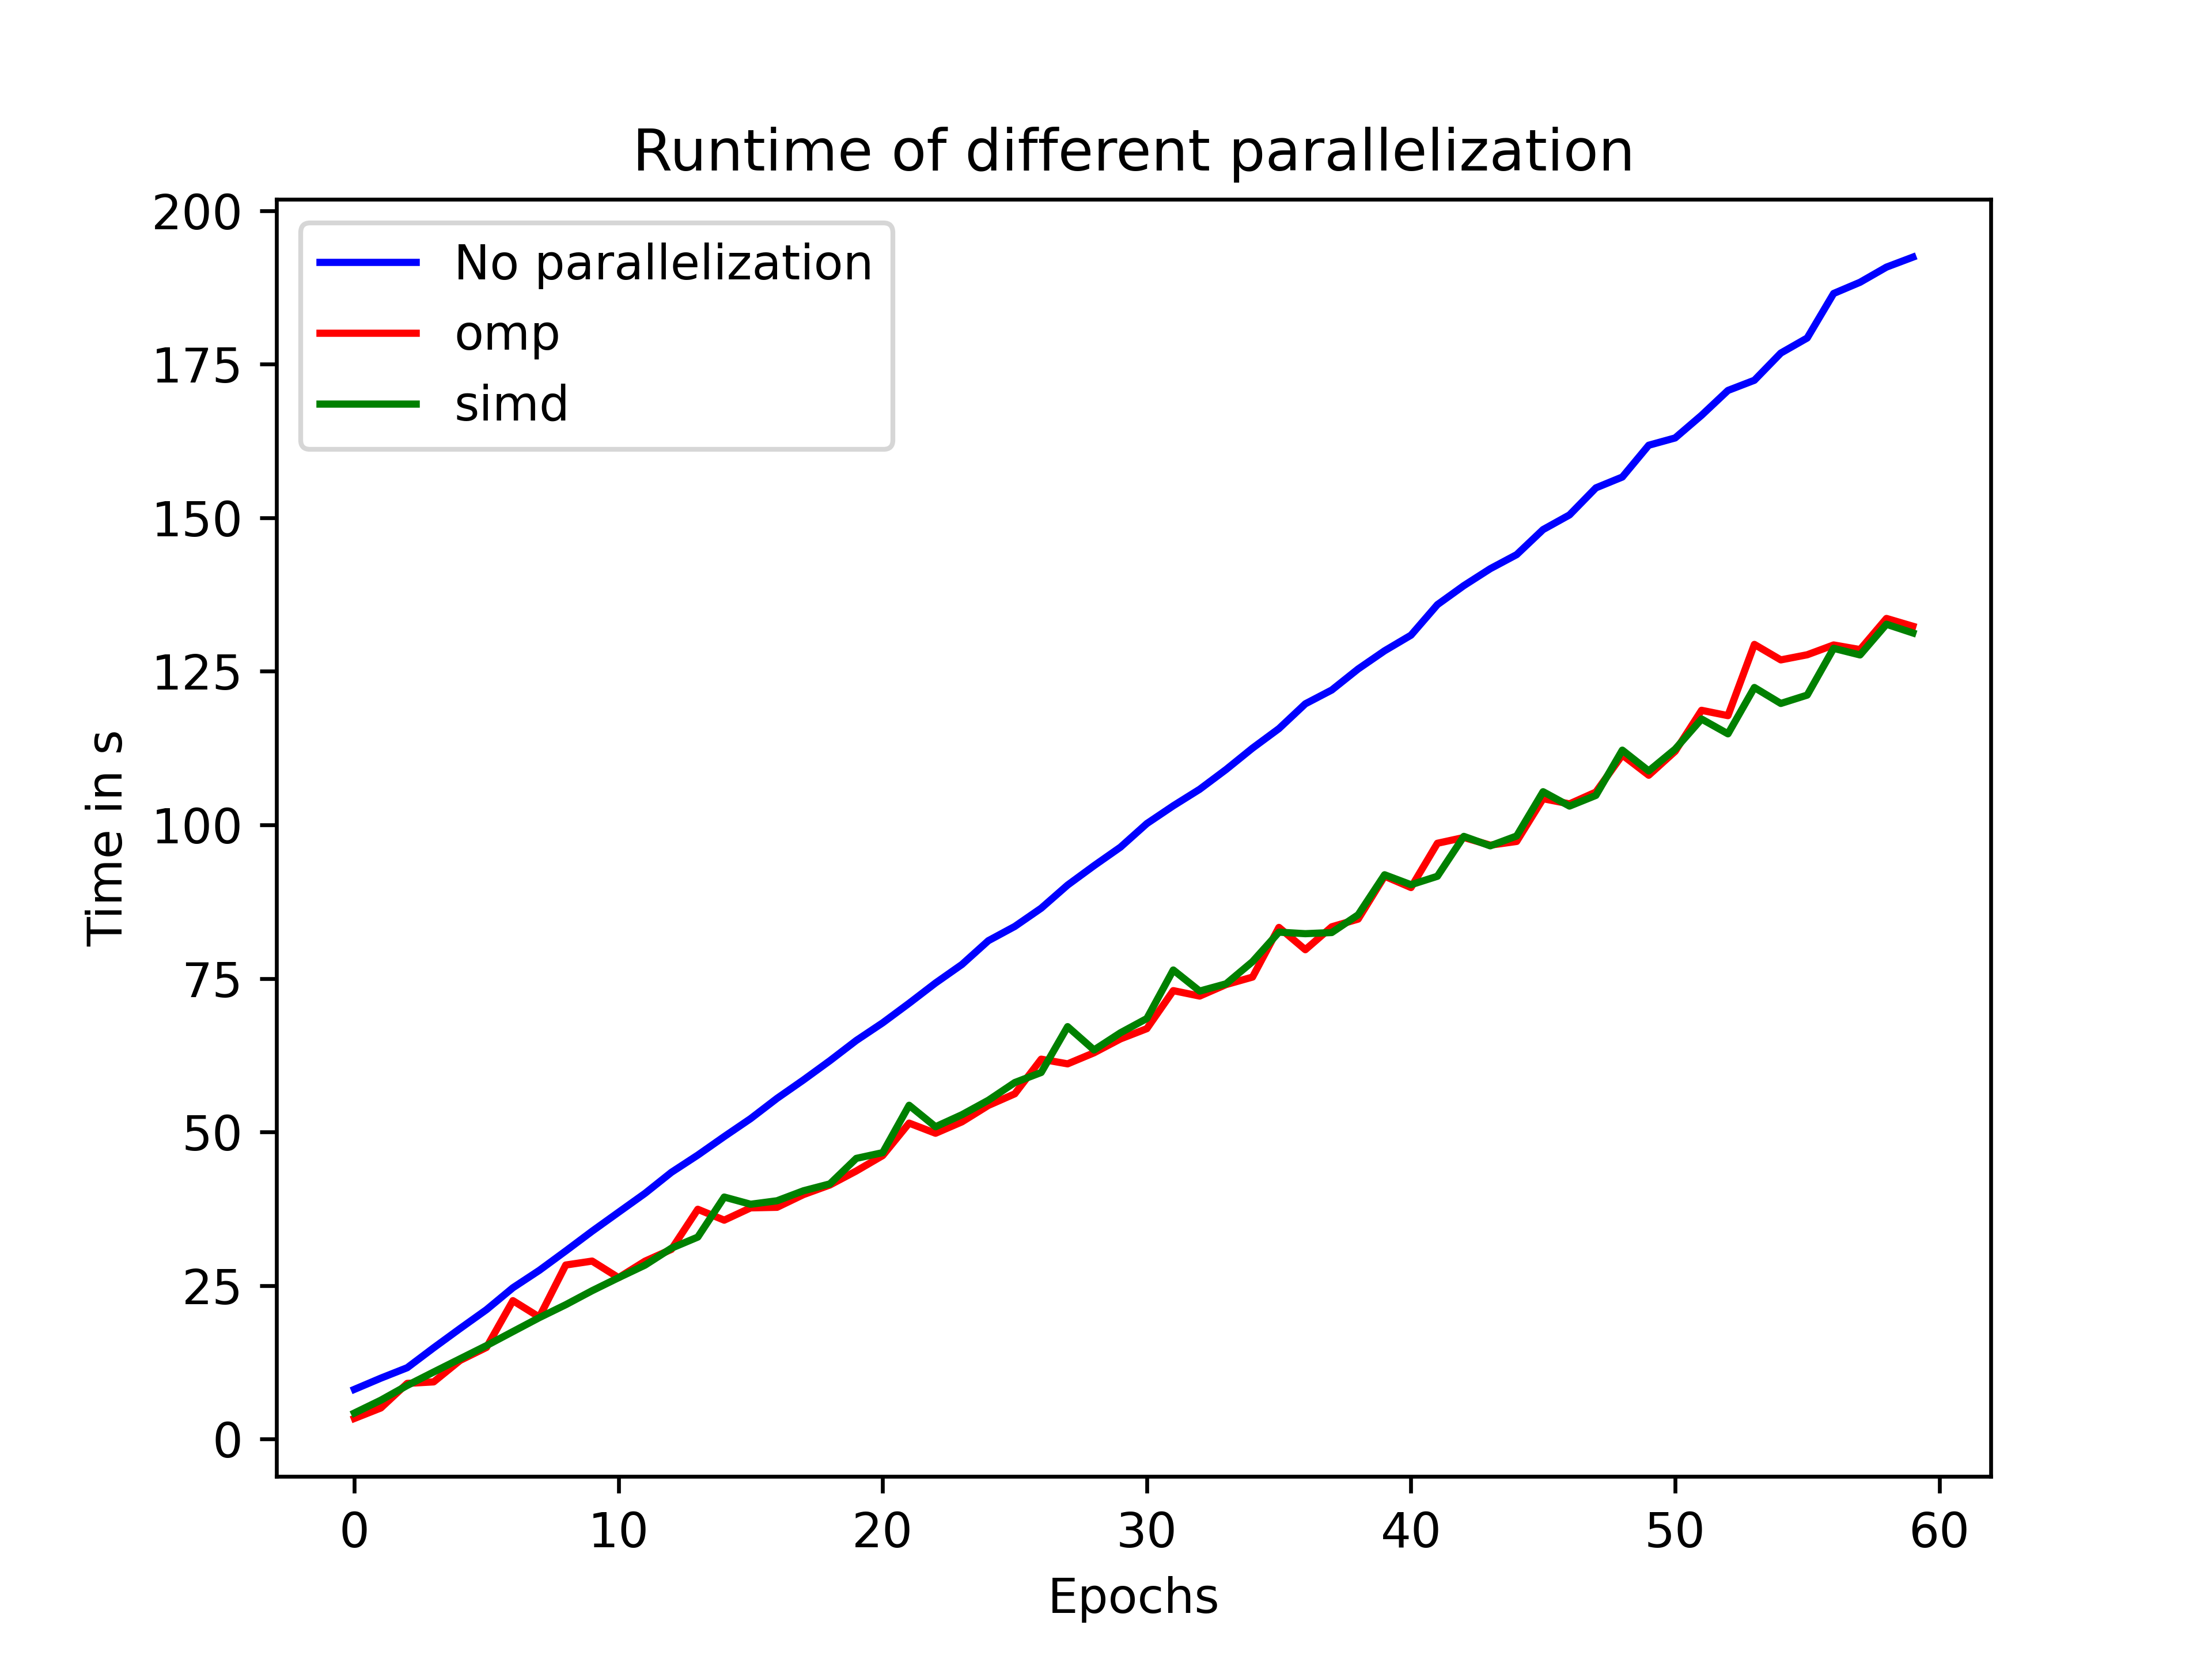
\includegraphics[width=9cm]{graphs/runtime_single.png}
	\caption{Vergleich der Laufzeit zwischen sequentiell, OMP und SIMD} \label{runtime single}
\end{figure}



\begin{figure}[h]
	\centering
	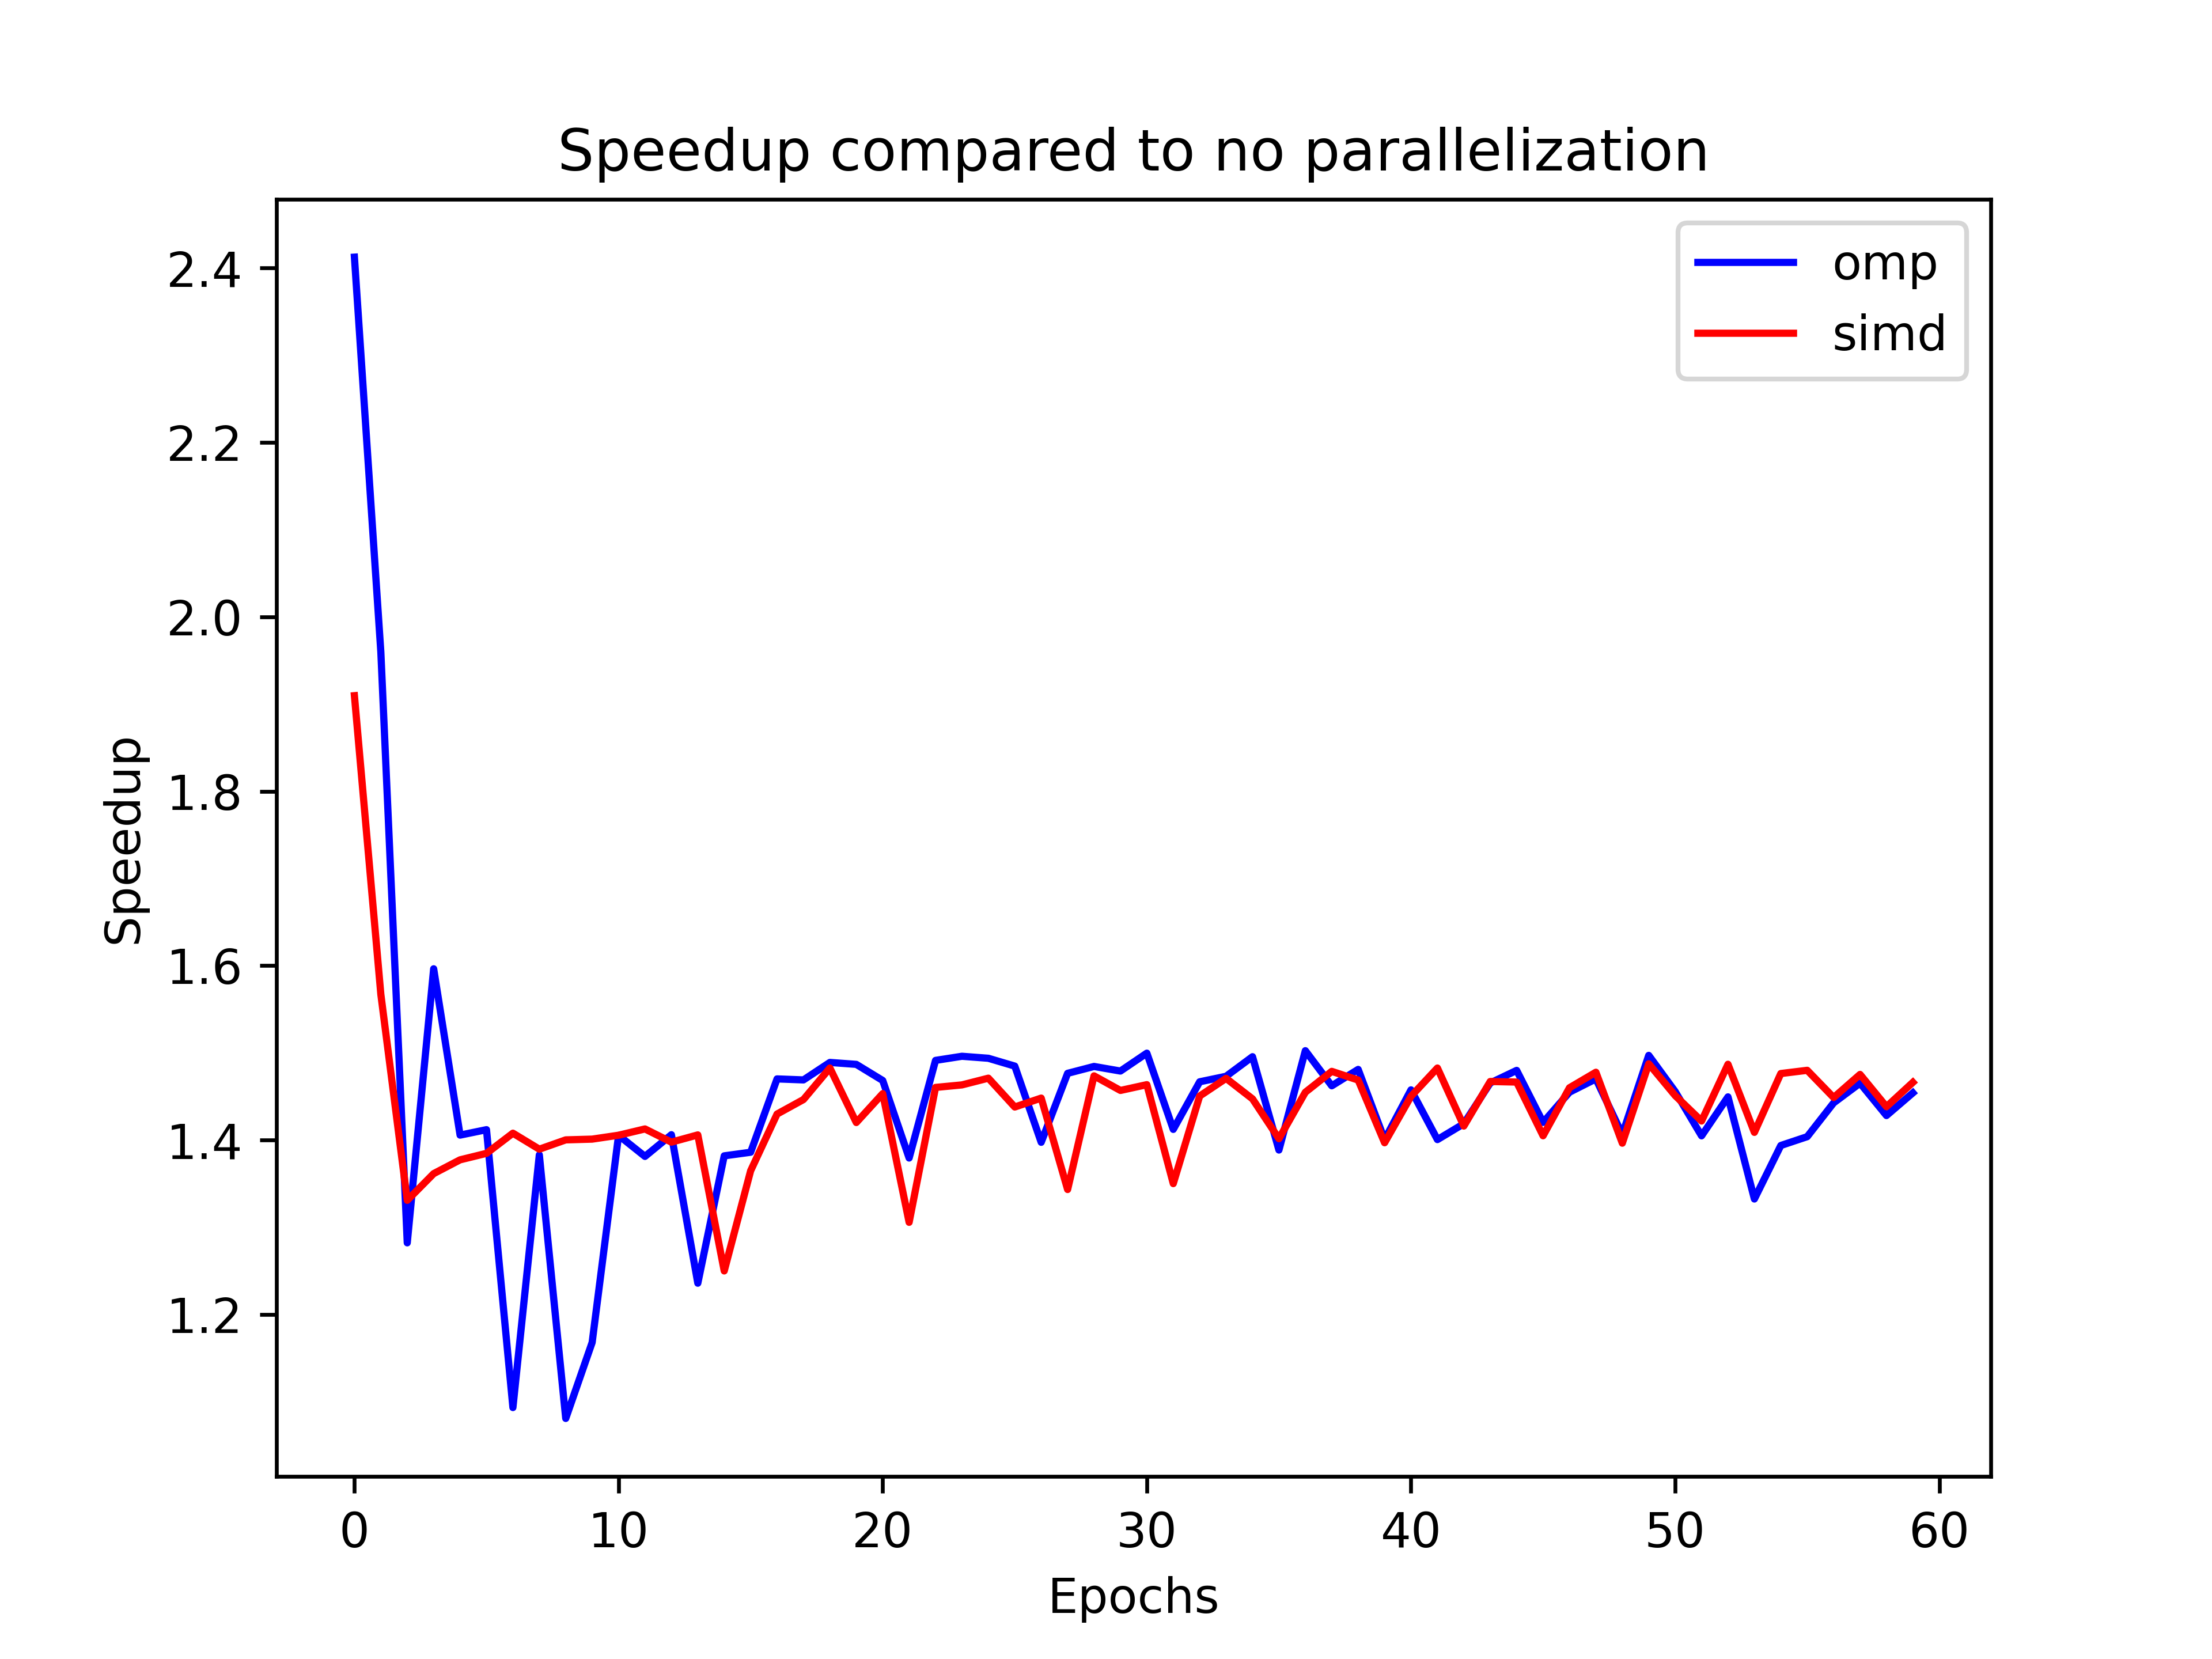
\includegraphics[width=9cm]{graphs/speedup_single.png}
	\caption{Vergleich des Speedups zwischen OMP und SIMD} \label{speedup single}
\end{figure}



\begin{figure}[h]
	\centering
	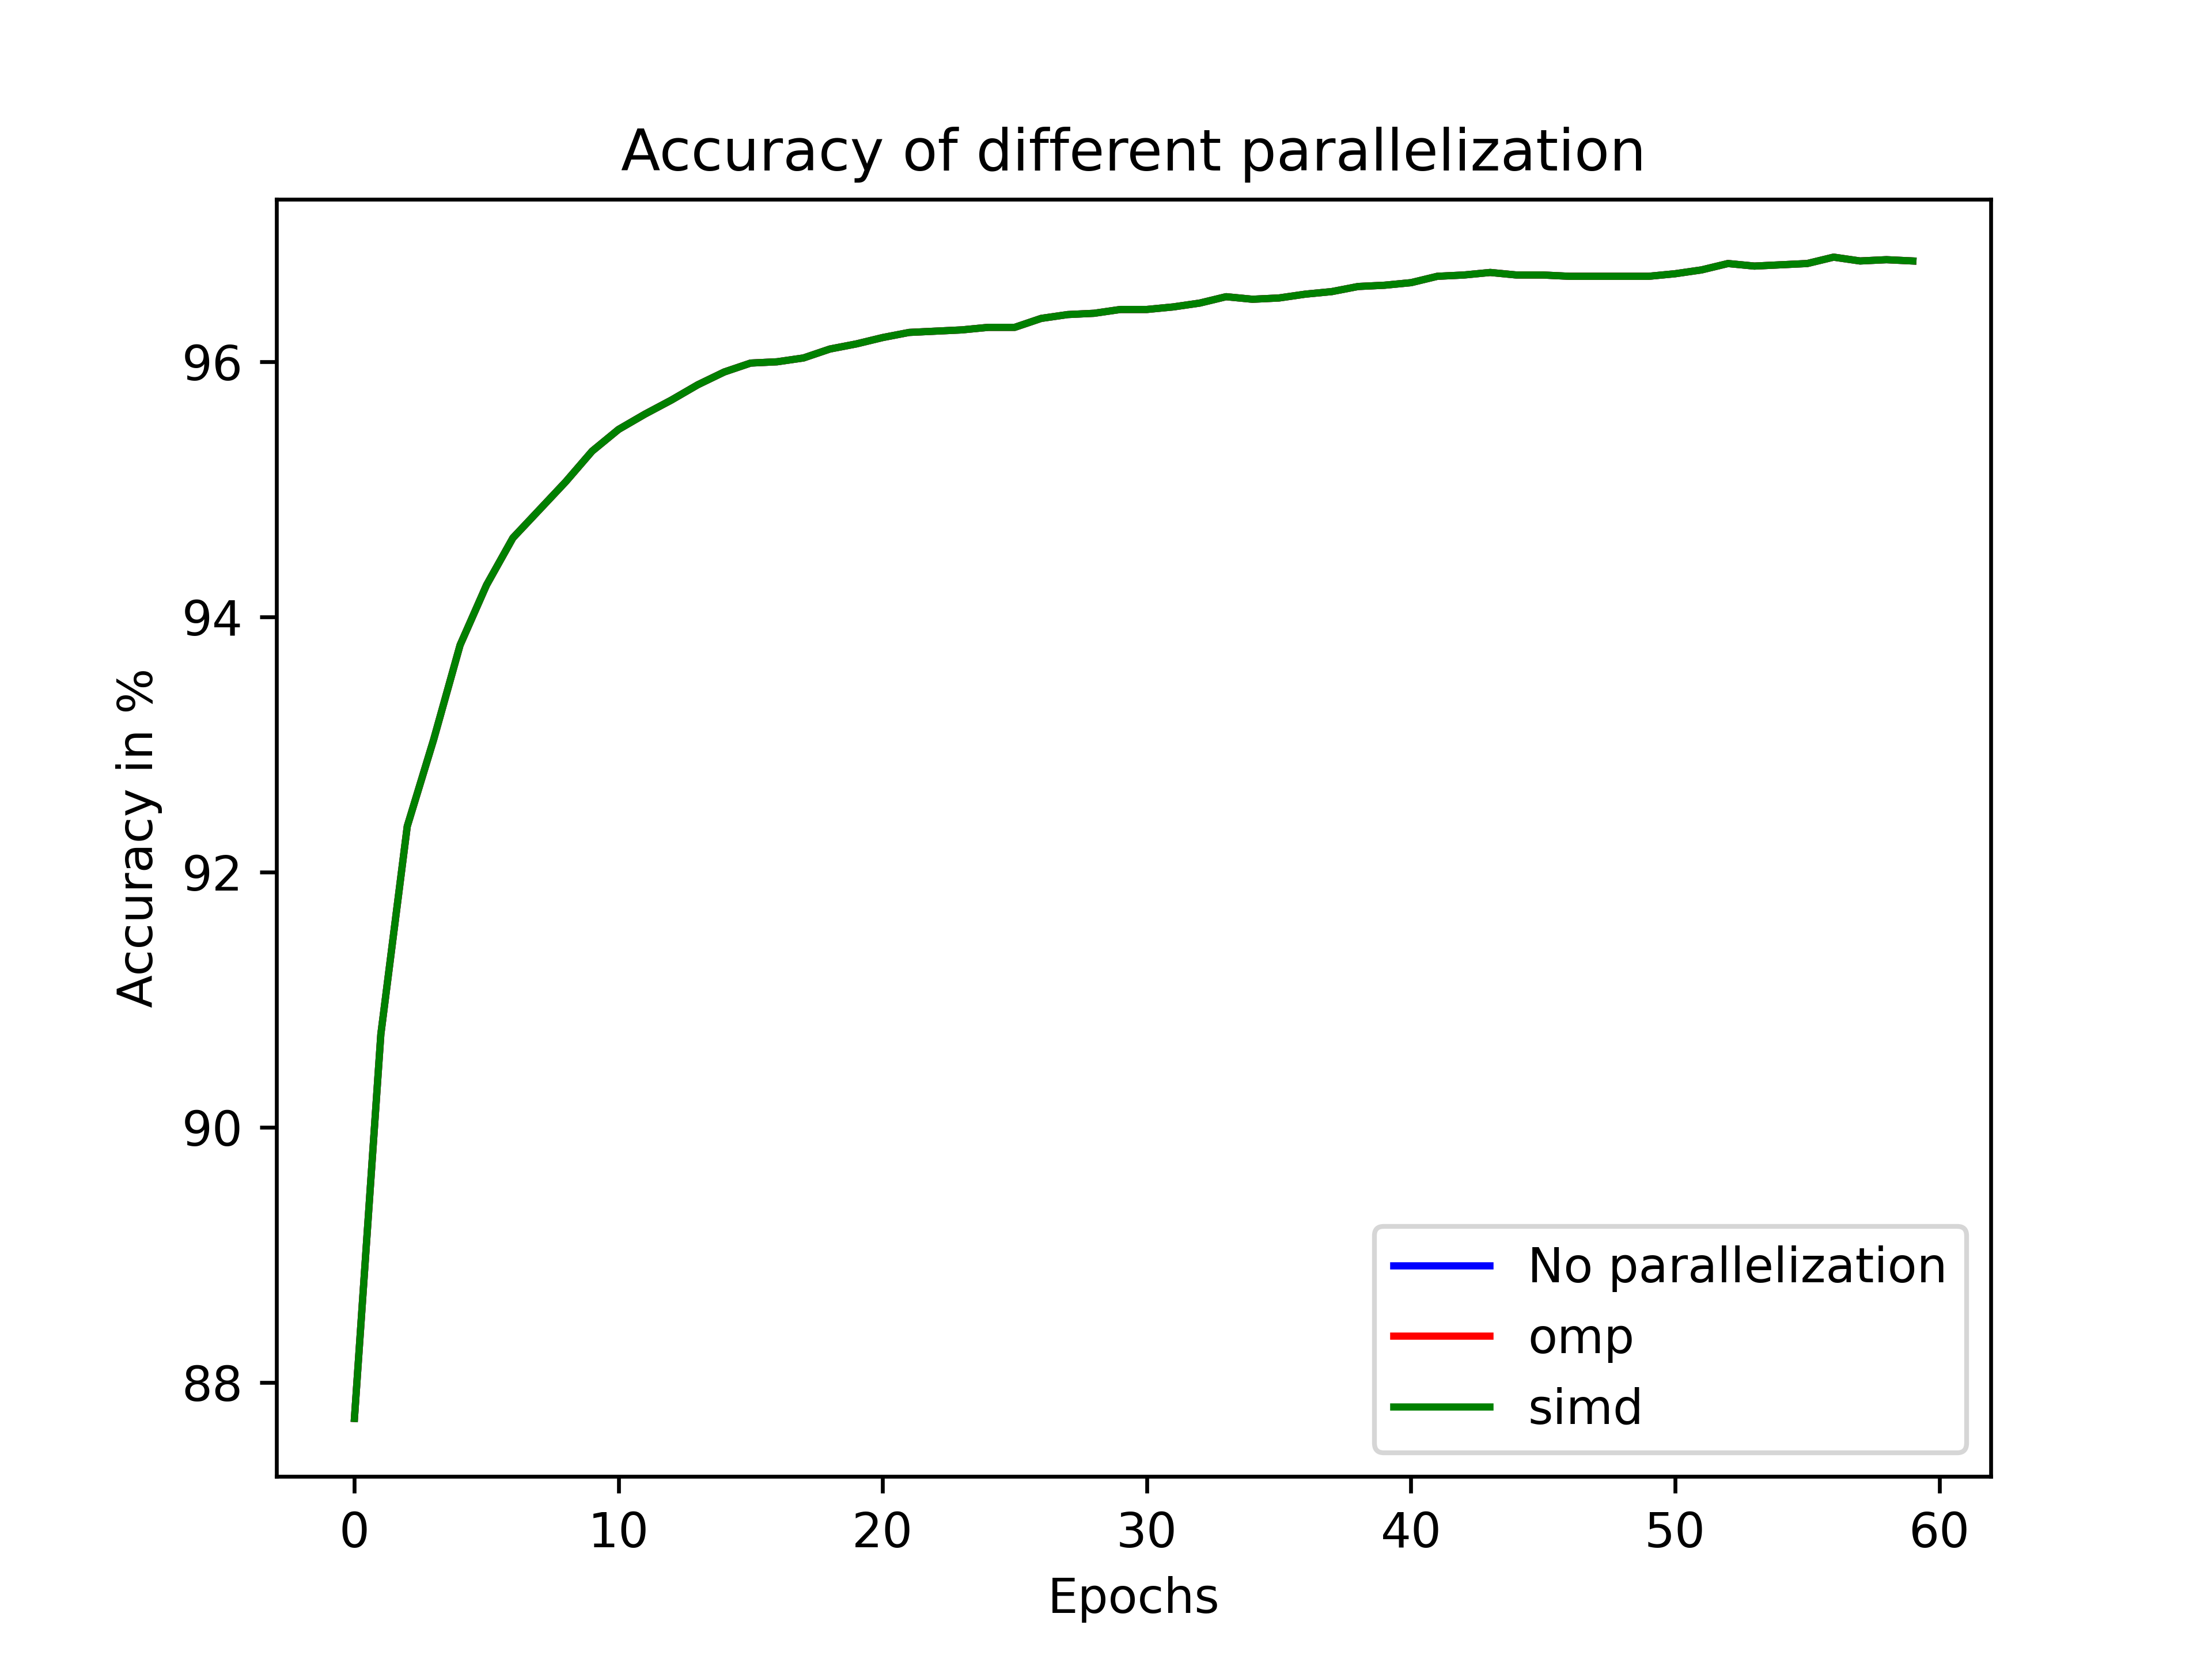
\includegraphics[width=10cm]{graphs/accuracy_single.png}
	\caption{Vergleich der Genauigkeit zwischen sequentiell, OMP und SIMD} \label{accuracy single}
\end{figure}
Als letztes m"ochten wir noch auf die Genauigkeit des Netzes eingehen. Im folgenden Graph in Abbildung \ref{accuracy single} l"asst sich diese gut veranschaulichen. Wie man sehen kann, steigt die Genauigkeiten in den ersten 10 Epochen sehr stark an und f"angt dann langsam an bei ca. 97 Prozent zu stagnieren. Dies ist bei allen drei Implementierung identisch. Leider muss man sagen, dass 97 Prozent keine gute Genauigkeit f"ur ein Neuronales Netz ist, wir es jedoch nicht geschafft haben eine h"ohere Genauigkeit zu erreichen. An der Stelle h"atte mit man mit umfangreichen Tests zu s"amtlichen Parametern, wie zum Beispiel Lernfaktor, Batch Size oder Gr"o\ss e und Anzahl der Hidden Layer, ein genaueres Ergebnis erzielen k"onnen. \\

\pagebreak

\section{Umsetzung}

Die theoretische L"osung sowie der Aufbau des geplanten Neuronalen Netzt muss nun ausgef"uhrt werden. Da das niemand h"andisch machen will, wird daf"ur eine Software L"osung ben"otigt.\\

Wie eingangs erw"ahnt nutzen wir f"ur den Code des Algorithmus die Programmiersprache C. Die Vorteile von C in diesem Projekt sind neben einer hohen Portabilit"at auch die M"oglichkeit schnelle und ressourcensparende Programme zu schreiben. Durch diese Vorteile eignet sich C am besten f"ur dieses Projekt. Als Compiler verwenden wir GCC, ein Open-Source Compiler-Suit der im Rahmen des GNU-Projektes entwickelt wird. Dieser ist auf den meisten Systemen anwendbar und steht kostenlos zur Verf"ugung.\\

Zu erst wird der simplere Teil des Netzes implementiert, das Berechnen des Outputs. Dabei gehen wir vorw"arts "uber die Schichten bis hinzu dem Output. Daf"ur starten wir in dem ersten Layer, dem Input, und berechnen wir f"ur jeden Knoten der darauffolgenden Schicht das Kreuzprodukt aus dem Input und der jeweiligen Gewichtungen zwischen den Knoten. Das Ergebnis wird daraufhin an die Aktivierungsfunktion "ubergegeben, bei uns die Sigmoidfunktion, und der Bias addiert. So gelangen wir zum Output, die Funktion wir auf Grund des "'vorw"arts durchgehen"' in den meisten Literaturen FeedForward genannt.\\

\begin{lstlisting}[language=C]
// code snippet from the inner for loop
nodes[row][layer + 1][node] = sigmoid(dotProduct(nodes[row][layer],net->weights[layer][node], net->n_nodes[layer]) + net->biases[layer][node]);
\end{lstlisting}

\pagebreak

Am Anfang wird ein Neuronales Netz mit einem zuf"alligen Werten f"ur die Gewichtungen initialisiert, damit ein Startpunkt kreiert werden kann. Doch dadurch ist das Ergebnis auch zuf"allig und der Algorithmus r"at eigentlich nur. Damit er nun auch tats"achlich seinen Input erkennt und wei\ss wie der Output sein sollte, muss das Programm "lernen".\\

F"ur eine bessere Verst"andlichkeit wird hier das Beispiel der Zahlenerkennung benutzt. Das Programm bekommt eine Zahl als Input und soll diese erkennen. Das Ergebnis wird dann mit eigentlichen Wert verglichen.\\
 
F"ur ein gut trainiertes Netz wird ein guter Lern-Datensatz ben"otigt, denn ein Netz wird nur das erkennen, was es so "ahnlich schon mal gesehen hat. Hier wird der MNIST Datensatz benutzt, dieser enth"alt 60.000 Trainingsbilder und 10.000 Testbilder und steht zur freien Verf"ugung.\\

\subsection{Perceptron}

Um in die Welt der neuronalen Netze einzutauchen und deren Lernweise zu verstehen, eignet sich das Perceptron. Da es auf zwei Layer reduziert ist, besteht es nur aus einer Input Schicht, die direkt mit einer Output Schicht verbunden ist (siehe Abbildung \ref{perceptron_pic}). Dadurch besteht ein direkter, linearer, Zusammenhang zwischen dem Input und den Output und es gibt nur einen Wert den wir anpassen k"onnen, die Gewichtungen der Verbindungen (siehe Deltalearn auf Seite \pageref{deltalearn_text}).\\

\begin{lstlisting}[language=C]
// inner loop from delta Learn
weights[i_output][i_input] += derivedSigmoid(noutputs[train_row] [i_output]) * train_image_data[train_row][i_input] * earn_rate * -2 * (outputs[train_row][i_output] - train_label_data[train_row][i_output]);
\end{lstlisting} 

Die Differnz gibt also die Richtung an in die die Gewichtungen angepasst werden, die weiteren Werte geben die St"arke an in der die Gewichtung ge"andert werden soll.\\

\subsection{Implementation der Hidden Schicht}

Die Anzahl der Gewichtungen war bis jetzt noch von der Anzahl der Inputs und Outputs abh"angig und auch auf diese begrenzt. Das Perceptron wird nur besser, wenn es ein gr"o\ss eres Bild als Input erh"alt. Damit das Neuronale Netz besser wird ohne den Input zu ver"andern, muss die Lernfunktion nicht linear werden (siehe Backpropagation auf Seite \pageref{backprop_text}).\\

Durch die Implementierung der Hidden Schicht erlangt das Netz eine deutlich h"ohere Komplexit"at, da so wie der Lernalgorithmus aufgebaut ist, nur bei einer direkten Verbindung zwischen Input und Output die Gewichtungen richtig angepasst werden k"onnen.\\

Der bestehende Algorithmus kann mit wenig "Anderung weiterhin verwendet werden um die Gewichtungen anzupassen die in den Output f"uhren. Die Gewichtungen die noch zwischen den Schichten davor sind, sollen auch angepasst werden, da so erst ein geringerer Fehler erreicht werden kann.\\

Das nach hinten "'weiterreichen"' der Differenz zwischen Output des Netzes und des Soll-Wertes, die Backporpagation, l"asst sich auch "ahnlich in Code umsetzten. Der Knoten vor dem Output bekommt seinen eigenen Fehlerwert, wie der Output auch einen hatte. Das wird, wie (Verweis einf"ugen) schon beschrieben, dadurch erreicht, dass alle Gewichte der ausgehenden Verbindungen des Knoten mit dem Fehler des Knoten auf mit dem sie verbunden sind multipliziert werden. Das geht dann solange weiter bis der Input erreicht wird.\\

Nach dem nun alle Fehler f"ur die einzeln Knoten berechnet wurde, werden diese wieder auf alle eingehenden Gewichtungen der jeweiligen Knoten addiert. 




\begin{lstlisting}[language=C]
//learn_factor init with 0 
void deltaBackProp(){
	for (int layer = n_layer - 2; layer > 0; layer--){
		for (int node = 0; node < n_nodes[layer]; node++){
			for (int past_node = 0; past_node < n_nodes[layer + 1]; past_node++) 
				{learn_factors[layer - 1][node] += learn_factors[layer][past_node] 
				* weights[layer][past_node][node];
			}
			learn_factors[layer - 1][node] *= 
				derivedFunktion(nodes[row][layer][node]);
		}
	}
}
\end{lstlisting}



\subsection{Batch Learning}

Diese Routine wird jetzt auf jede Datensatz angewendet, das sind bei MNIST-Datensatz 60.000 Wiederholungen. In jeder Wiederholung muss erst FeedForward ausgerechnet werden, um dann den errechneten Output mit seinem Fehler zur"uckzupropagieren.\\

Die momentane Implementation ist mit Memory Spielen zu vergleichen, wir drehen eine Karte um und wenn wir falsch liegen m"ussen wir uns merken welche Karte wo lag. Nur das dieses Spiel aus 60.000 P"archen besteht, wir werden also nie mit nur einem Versuch ein richtiges P"archen finden, aber unsere Trefferquote w"urde sich verbessern, wenn wir mit einem Zug immer mehrere Felder auf Einmal umdrehen d"urften.\\

Bei dem kleinen Gedankenspiel w"urde die Menge an Daten, die sich gemerkt werden m"ussen, zwar nicht weniger werden, aber die Anzahl an Runden w"urde sich verringern. Dieser Gedanke l"asst sich auch auf den Lernalgorithmus anwenden. \\

\pagebreak

Der Datensatz wird in Stapel, sogenannte Batches, unterteilt. Bevor ein Stapel angeschaut wird, wird FeedForward angewendet, danach werden die Ergebnisse wieder mit den Sollwerten verglichen und die Gewichte abgepasst. Wie im Beispiel schauen wir uns nicht weniger Daten an und m"ussen auch nicht weniger Gewichtungen lernen, aber durch das Batchlearning erreichen wir schneller eine geringe Fehlerrate und minimieren auch den Zufallseffekt, der einzelnen Datens"atze.\\

Der kleinste Stapel w"are also ein einzelnes Datenpaar und der gr"o\ss te w"are der gesamte Datensatz. Je gr"o\ss er der Batch, umso genauer ist jede Anpassung pro Epoche und die Fehlerminimierung gleicht fast dem Gradientenabstieg. Es auch werden zuf"allig Spr"unge, die das Netz auch verschlechtern k"onnen, vermieden. Allerdings ist dadurch die Anpassung an den Gewichtungen auch nur minimal, es werden also mehr Epochen ben"otigt. Die Wahl der Batch Size ist ein Zusammenspiel von der gew"unschten Genauigkeit und der Geschwindigkeit, mit der diese erreicht werden soll.\\

\subsection{Graphical User Interface}
Zus"atzlich zu einer terminalbasieten Ausf"uhrung des Programms hatten wir uns zudem noch als Ziel gesetzt, eine grafische Benutzeroberfl"ache zu implementieren, da dies einige Vorteile mit sich bringt.
Zum Einen ist es f"ur den Benutzer deutlich intuitiver eine graphische Anwendung zu bedienen, als das Programm "uber das Terminal aufzurufen. Au\ss erdem wollten wir dem Benutzer die M"oglichkeit geben, das neuronale Netz mit einer eigens angefertigten Skizze zu testen, sodass das Ergebnis des Netzes direkt in der GUI angezeigt werden kann. Wir einigten uns darauf, dies in Python mit Tkinter umzusetzen, da wir darin die meiste Erfahrung hatten. Aufgebaut ist unsere GUI wie folgt:\\

\begin{figure}[h]
	\centering
	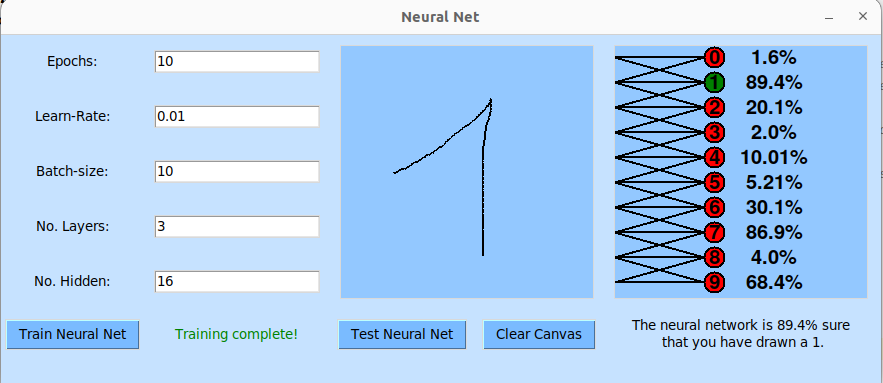
\includegraphics[width=10cm]{screens/gui.png}
	\caption{Screenshot der Grafischen Oberfl"ache} \label{screen_gui}
\end{figure}

Wie in dem Screenshot zu sehen, ist unsere GUI grob in drei Segmente aufgeteilt. Auf der linken Seite befinden sich die wesentlichen Parameter des neuronalen Netzes. Diese kann der Benutzer selber in die Eingabefelder eintragen und mittels eines Klicks auf den darunterliegenden Button das neuronale Netz mit diesen trainieren. 

\pagebreak

Als Feedback, ob das trainieren erfolgreich war, wird ein kleiner Text rechts von dem Button eingeblendet.\\

Anschlie\ss end befindet sich in der Mitte der GUI eine leere Leinwand, auf der der Benutzer mit der Maus eine Ziffer malen kann. Diese Skizze wird zun"achst in einem 252 $ \cdot$ 252 Numpy Array gespeichert. Da das neuronale Netz aber nur 28 $\cdot$ 28 Arrays als Input akzeptiert mussten wir noch digitale Bildbearbeitung anwenden. Dazu bot sich die OpenCV Bibliothek an. Diese beinhaltet verschiedenste Algorithmen f"ur die Bildbearbeitung und Computer Vision. Wir ben"otigten f"ur unseren Anwendungsfall jedoch nur die resize()-Funktion, bei der ein Bild-Array auf ein beliebig gro\ss es Array angepasst werden kann. Wichtig daf"ur ist die Art der Interpolation, wir entschieden uns f"ur "'INTER\_ AERA"', da diese das Array unter Verwendung des Pixelfl"achenverh"altnisses resampled. \\

\begin{figure}[h]
	\centering
	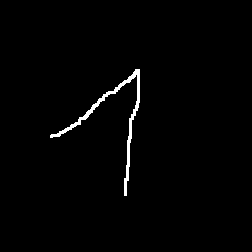
\includegraphics[width=6cm]{screens/BILD252x252.png}  \hfill
	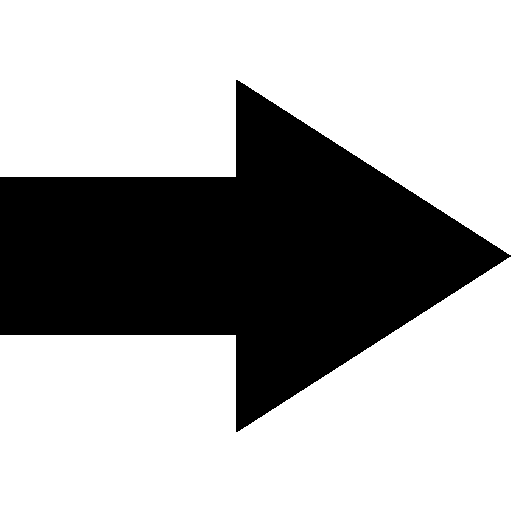
\includegraphics[width=3cm]{screens/arrow.png} \hfill
	
\includegraphics[width=6cm]{screens/BILD28x28.png}
	\caption{Downscaling des 252 $\cdot$ 252 Bildes auf 28 $\cdot$ 28 Pixel} \label{28x28}
\end{figure}


Anschlie\ss end wird das neue Array als csv-Datei gespeichert und von dem neuronalen Netz eingelesen und getestet. Liegen nun die Ergebnisse vor, werden diese in der Grafik auf der rechten Seite der GUI angezeigt. Mit unserem Aufbau der GUI und des Netzes l"asst sich das Netz beliebig oft testen, ohne jedes Mal das Netz neu trainieren zu lassen.

\pagebreak

\section{Fazit}

Letztendlich ist es uns gelungen ein neuronales Netz ohne Bibliotheken Dritter zu implementieren. Es erkennt, wie erwartet, den Gro\ss teil der Zahlen aus den MNIST Datens"atzen. Der Einstieg in ein so komplexes Thema war schwierig, vor allem da keiner von uns Erfahrungen mit neuronalen Netzen hatte. Auch nach einiger Recherche und den ersten Vorlesungen zu diesem Thema war uns unklar wie wir anfangen sollten. Doch mit Hilfe des simplen Perceptrons haben wir erfolgreich die ersten Schritte gemeistert.\\

Von diesem Punkt an ging die Entwicklung stetig voran, doch die Parallelisierung mit SIMD bereitete uns bis zum Schluss Probleme, da sie im Gegensatz zu OMP nicht einfach hinzugef"ugt werden konnte. Stattdessen musste man es von Anfang an auf komplexe Weise in den Code und die Berechnungen integrieren, was uns nicht gelungen ist. Die Implementierung und Verwendung von OMP war jedoch erfolgreich, so dass das Netz deutlich k"urzere Laufzeiten hatte.\\

Obwohl nicht alle Anforderungen erf"ullt wurden, haben wir dennoch eine Menge w"hrend diesem Semesterprojekt gelernt. Zum einen "uber das aktuelle Thema machine Learning, welches heutzutage in fast s"amtlichen Bereichen Anwendung findet. Zum Anderen "uber die Parallelisierung von Programmen gelernt, welche es erlaubt rechenintensiven Code schneller ausf"uhren zu lassen und so die Wartezeiten zu verk"urzen. 

\pagebreak

\begin{thebibliography}{99}
  \bibitem{SIMD}{\url{https://gitlab.htw-berlin.de/bauers/ce20-mpt-sose-22/-/blob/main/slides/03-simd.pdf}} \label{bauer_simd}
  
  \bibitem{k_netz}{\url{https://de.wikipedia.org/wiki/K\%C3\%BCnstliches_neuronales_Netz}} \label{wiki_k_netz}
  
  \bibitem{k_neuron}{\url{https://de.wikipedia.org/wiki/K\%C3\%BCnstliches_Neuron}} \label{wiki_k_neuron}
  \bibitem{delta_learn_wiki}{\url{https://en.wikipedia.org/wiki/Delta_rule}} \label{delta_learn_wiki}
  \bibitem{codecamp_howto_net}{\url{https://www.freecodecamp.org/news/building-a-neural-\
  network-from-scratch}} \label{codecamp_howto}  
  
  \bibitem{datasolut_ki_einsatz}{\url{https://datasolut.com/anwendungsgebiete-von-kuenstlicher\
  intelligenz/#Robotik}} \label{ki_einsatz}

  \bibitem{c_vorteile}{\url{https://www.it-treff.de/it-lexikon/c-programmiersprache}} \label{c_vorteile}

\bibitem{c_vorteile}{\url{https://www.kaggle.com/code/residentmario/full-batch-mini-batch-and-online-learning/notebook}} \label{c_vorteile}

  
  \bibitem{sigmoid}{\url{https://www.allaboutcircuits.com/technical-articles/sigmoid-activation-function-activation-in-a-multilayer\
  -perceptron-neural-network/}} \label{sigmoid_src}
  
  \bibitem{backprop}{\url{https://deepai.org/machine-learning-glossary-and-terms/backpropagation}} \label{backprop}
  \bibitem{youtube_from_scratch}{\url{https://www.youtube.com/watch?v=Wo5dMEP_BbI&list=PLQVvvaa0QuDcjD5BAw2DxE6OF2tius3V3}} \label{youtube_from_scratch}
  \bibitem{youtube_deltalearn}{\url{https://www.youtube.com/watch?v=4E4GhVREXBg&list=PL58qjcU5nk8sUq97ze6MZB8aHflF0uNgK&index=10}} \label{youtube_deltalearn}
  
\end{thebibliography}

\end{document}
